\documentclass[
	english,
        solution=true
	]{tudaexercise}

\usepackage[main=english, ngerman]{babel}
\usepackage[babel]{csquotes}

\usepackage{amstext}
\usepackage{amsmath}
\usepackage{amssymb}
\usepackage{graphicx}
\usepackage{setspace}
\usepackage{multicol}
\usepackage{mathtools}
\usepackage{dsfont}
\usepackage{units}
\usepackage{subfigure}
\usepackage{color}
\usepackage{booktabs}
\usepackage{fancyref}
\usepackage{listings}
\usepackage{mathrsfs}
\usepackage{physics}
\usepackage{gauss}
\usepackage{bm}
\usepackage{multirow}
\usepackage{pgfplots}
\usepackage{pgfplotstable}
\usepackage{hyperref}
\usetikzlibrary{patterns}
\usepackage{wasysym}
\usepackage{enumitem}
\usepackage{caption}
\captionsetup{justification=centering}
\usepackage{tcolorbox}
\usepackage{fontspec}
\setmainfont{Aptos}
\usepackage{float}
\usepackage{hyperref}

\let\file\texttt
\let\code\texttt
\let\pck\textsf
\let\cls\textsf
\let\tbs\textbackslash

\newlist{checkboxes}{itemize}{1}
\setlist[checkboxes]{label=$\square$, leftmargin=*}

\newtcolorbox{programmingtaskbox}{
  colback=blue!5!white,
  colframe=lightgray!75!black,
  title=Programming Task,
  sharp corners,
  boxrule=0.8pt,
  leftrule=1mm
}

\ConfigureHeadline{
	headline={title}
}

\let\unit\relax

\newcommand{\R}{\mathbb{R}}
\DeclareMathOperator*{\argmax}{arg\,max}
\DeclareMathOperator*{\argmin}{arg\,min}

\begin{document}
\author{Prof. Marcus Rohrbach, Prof. Simone Schaub-Meyer}
\term{Summer Term 2025}
\title[Statistical Machine Learning Exercise 3]{\LARGE Statistical Machine Learning: Exercise 3}
\subtitle{Regression, Kernel Theory, Gaussian Processes, Latent Representation \\ Total Possible Points: 82}
\maketitle

\boxed{\textbf{Group 210}}\\
\textbf{Mateo Arenas}\\
\textbf{Diusne Olavide}

\begin{task}[points=34]{Regression}
    \begin{programmingtaskbox}
        Google Colab: \url{https://colab.research.google.com/drive/1kF9azPGS7ZNYaO0_rhi0_j-O6X-a27XU?usp=sharing}
    \end{programmingtaskbox}

    In this exercise, you will implement various kinds of linear regressors using the data \texttt{lin\_reg\_train.txt} and \texttt{lin\_reg\_test.txt}.
    The files contain noisy observations from an unknown function $f: \mathbb{R} \mapsto \mathbb{R}$.
    In both files, the first column represents the input and the second column represents the output.
    You can load the data using \texttt{numpy.loadtxt} and built-in functions for computing the mean.

    For all subtasks, assume that the data is identically and independently distributed according to
    \begin{equation*}
        y_i = \bm{\Phi}(\mathbf{x_i})^\top \mathbf{w} + \epsilon_i,
    \end{equation*}
    where
    \begin{equation*}
        \epsilon_i \sim \mathcal{N}(0, \sigma^2),
    \end{equation*}
    and $\Phi: \mathbb{R} \rightarrow \mathbb{R}^n$ is a feature transformation such that
    \begin{equation*}
        \mathbf{y} \sim \mathcal{N}(\bm{\Phi}(\mathbf{X})^\top \mathbf{w}, \sigma^2 \mathbf{I}).
    \end{equation*}

    Additionally, make sure that your implementations support multivariate inputs. The feature transformations
    are given in each task; if no basis function is stated explicitly, use the data as is, i.e.~$\bm{\Phi}(x) = x$.

    \begin{subtask}[points=8, title=Linear Features]
        Implement linear ridge regression using linear features, i.e.~the data itself by filling in the ToDos of the corresponding task in the provided Colab Template.
        Include an additional input dimension to represent a bias term and use the ridge coefficient $\lambda = 0.01$.
        
        \begin{enumerate}
            \item Explain: What is the ridge coefficient and why do we use it? 
            \item Derive the optimal model parameters by minimizing the squared error loss function. 
            \item Report the root mean squared error of the train and test data under your linear model with linear features. 
            \item Include the resulting plot and a short description. 
        \end{enumerate}

        \begin{solution}
            \textbf{1. Explain: What is the ridge coefficient and why do we use it?}

            In the lecture (Slide 42), the regularized least squares problem is introduced as the Maximum A-Posteriori (MAP) estimate in a Bayesian linear regression setting.
            The coefficient function is:

            \[
            w = \arg\min_w \frac{1}{2} \|\Phi^\top w - y\|^2 + \frac{\lambda}{2} \|w\|^2
            \]

            % Here, $\lambda = \sigma^2 / \sigma_0^2$ arises naturally from the ratio of observation noise variance $\sigma^2$ to prior variance $\sigma_0^2$ on the weights $w$.

            The term $\lambda$ controls the complexity of the model and determines the degree of overfitting.
            A smaller $\lambda$ allows the model to fit the training data more precisely, while a larger $\lambda$ reduces the overfitting.

            The objective is to avoid unstable "valleys".
            The ones that appear when using \textit{Least squares}, as seen in the figure \ref{Task1a_1}.

            \begin{figure}[H]
                \centering
                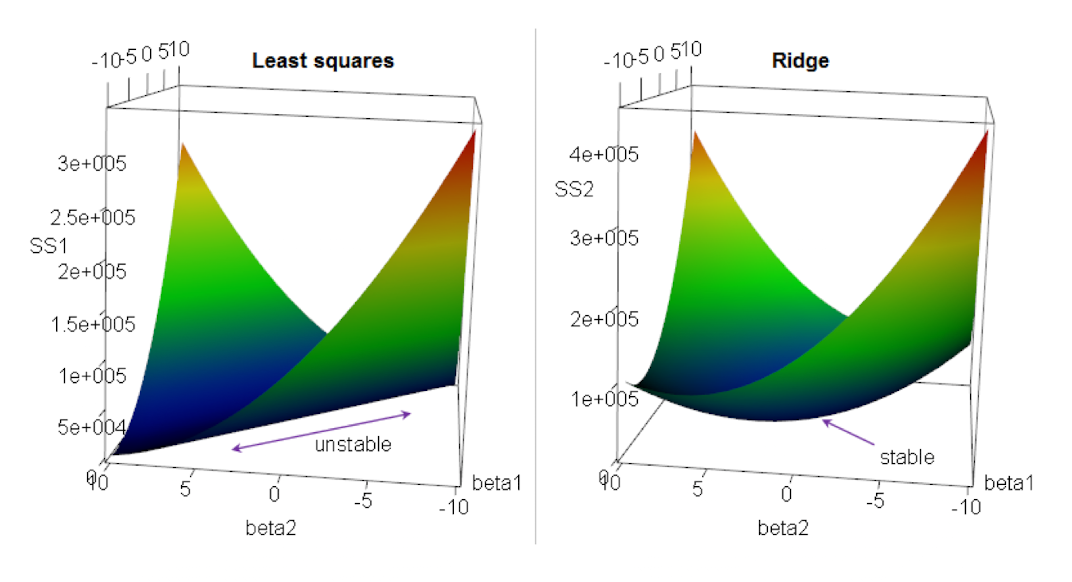
\includegraphics[width=0.5\textwidth]{images/Task1a_1.png}
                \caption{Example. The difference when using Ridge vs. Least squares}
                \label{Task1a_1}
            \end{figure}
            
            \vspace{2em}

            \textbf{2. Derive the optimal model parameters by minimizing the squared error loss function.}

            As shown in Slide 42 of the lecture, we minimize the regularized least squares loss:

            \[
            L(w) = \frac{1}{2} \|\Phi^\top w - y\|^2 + \frac{\lambda}{2} \|w\|^2
            \]

            Taking the derivative with respect to $w$ and setting it to zero:

            \[
            \frac{\partial L}{\partial w} = \Phi(\Phi^\top w - y) + \lambda w = 0
            \]

            Rearranging:

            \[
            \Phi \Phi^\top w + \lambda w = \Phi y
            \]

            Solving for $w$:

            \[
            w = (\Phi \Phi^\top + \lambda I)^{-1} \Phi y
            \]

            This is the closed-form solution for regularized linear regression (ridge regression).

            \vspace{2em}

            \textbf{3. Report the root mean squared error of the train and test data under your linear model with linear features.}

            The result of the RMSE of the train and test data for the linear model and features is the following:

            \vspace{1em}

            \textbf{\texttt{Linear Features}}
            \begin{itemize}
                \item \texttt{Train RMSE: 0.4122}
                \item \texttt{Test RMSE: 0.3843}
            \end{itemize}

            \vspace{1em}

            The RMSE values are relatively low and close to each other, indicating that the model generalizes well to unseen data and does not overfit.
            This is expected for a simple linear model with mild regularization on a smooth dataset.

            \vspace{2em}

            \textbf{4. Include the resulting plot and a short description.}

            \begin{figure}[H]
                \centering
                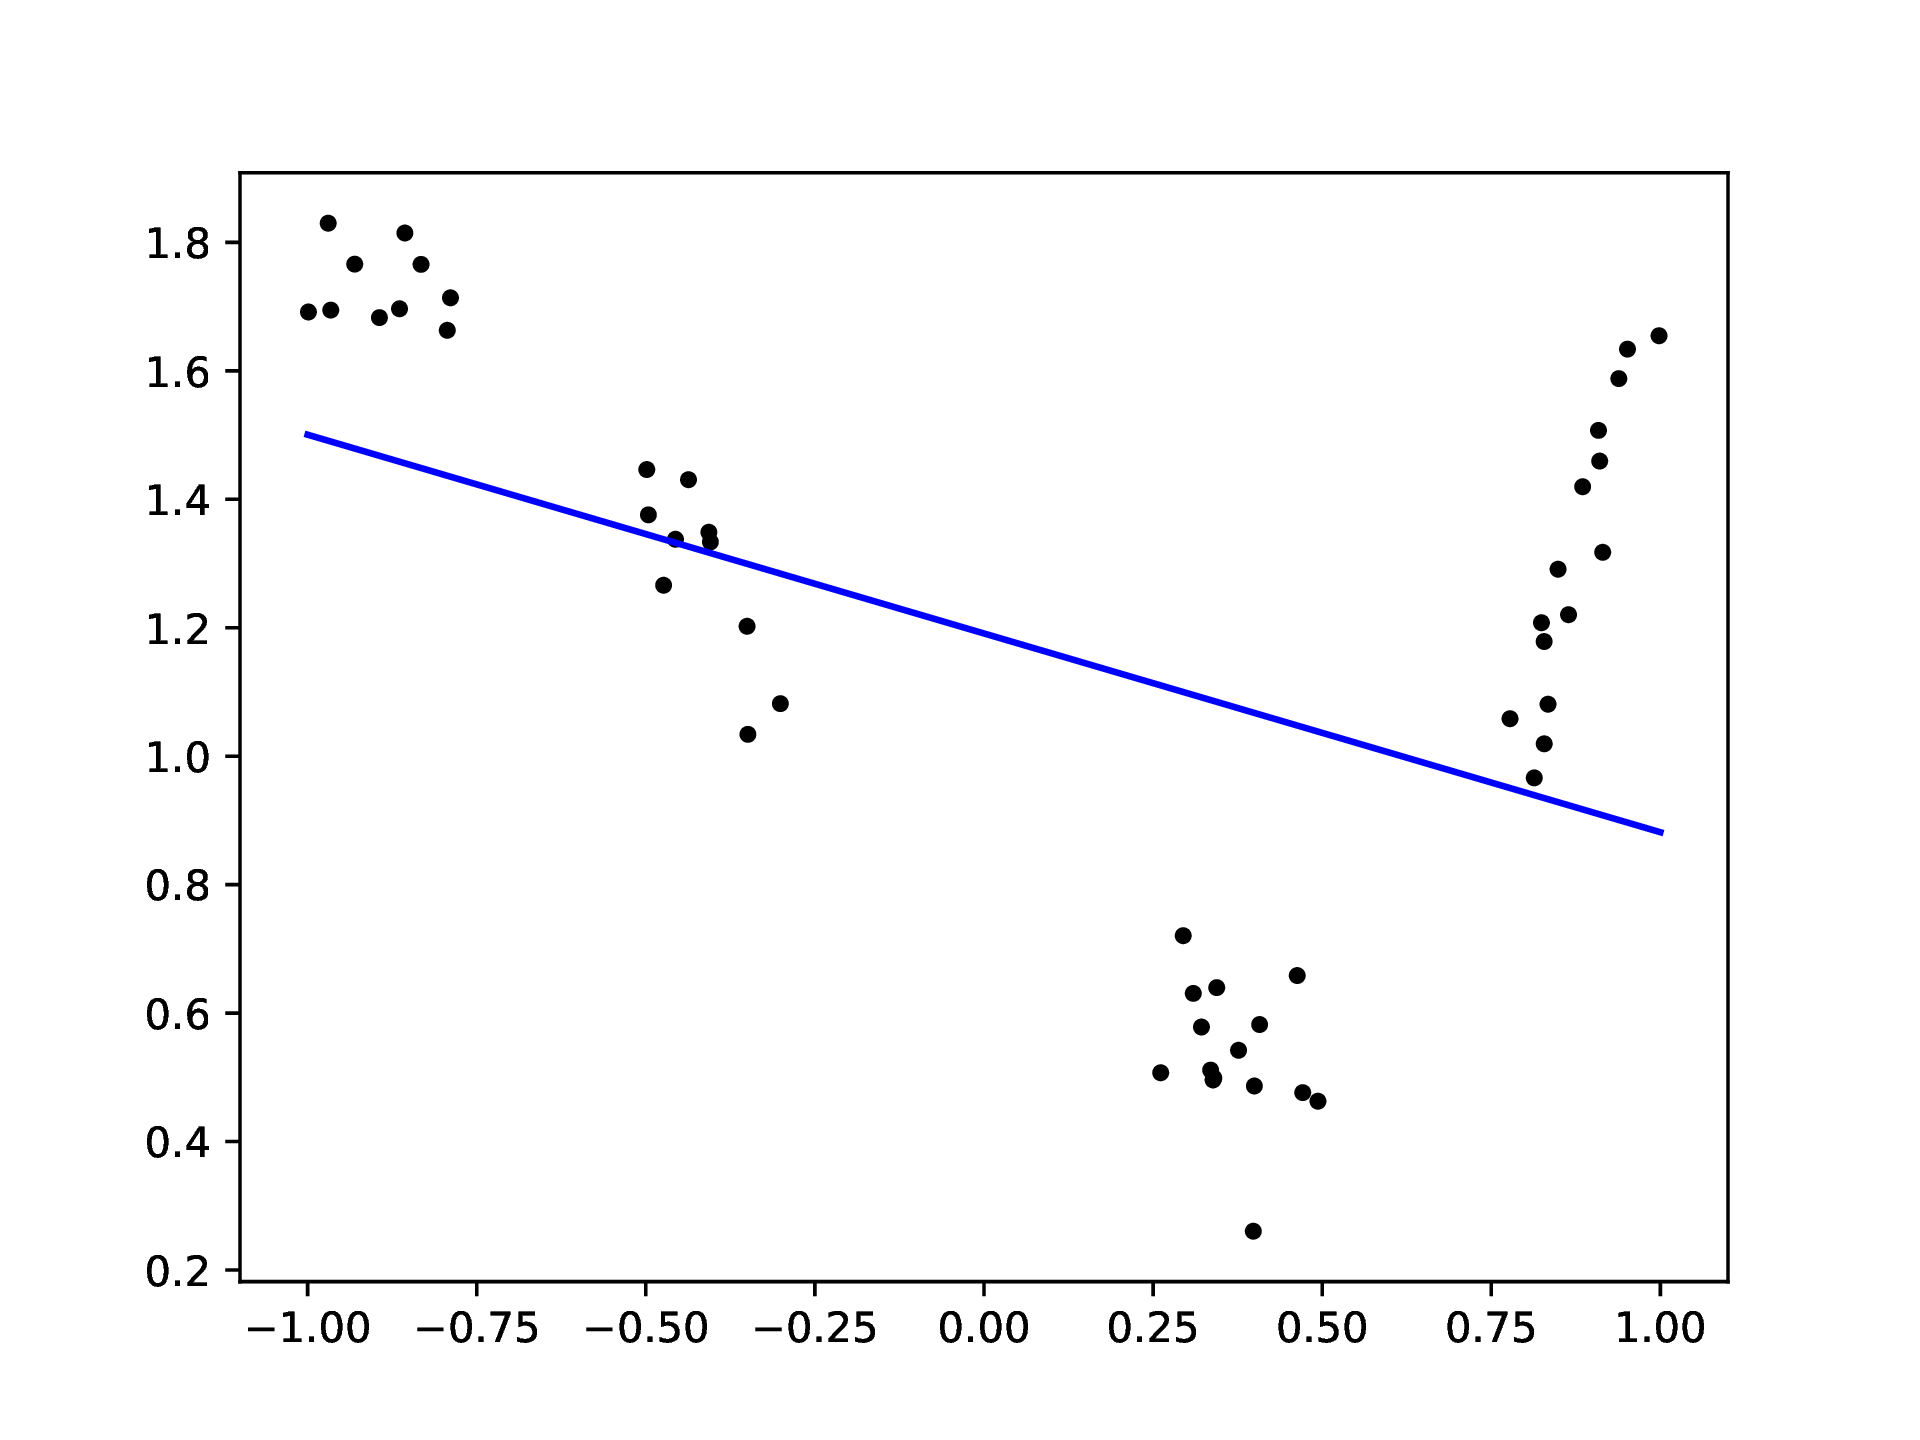
\includegraphics[width=0.5\textwidth]{images/Task1a_4.png}
                \caption{Linear ridge regression fit with $\lambda = 0.01$ using linear features and bias.
                % Black dots represent the data points. The blue line is the fitted regression model.
                }
            \end{figure}

            The model fits a straight line through the data. Since the data shows a clear nonlinear pattern, the linear model cannot capture it well.
            Still, the fit shows a general trend and does not overfit the noise, which explains the relatively low RMSE values.

        \end{solution}

    \end{subtask}

    \begin{subtask}[points=8, title=Polynomial Features]
        Implement linear ridge regression using a polynomial feature projection by filling in the ToDos of the corresponding task in the provided Colab Template.
        Include an additional input dimension to represent a bias term and use the ridge coefficient $\lambda = 0.01$.

        For polynomials of degrees 2, 3 and 4:

        \begin{enumerate}
            \item Report the root mean squared error of the training data and of the testing data under your model with polynomial features.
            \item Include the resulting plot and a short description.
            \item Why do we call this method \textit{linear} regression despite using polynomials?
        \end{enumerate}

        \begin{solution}
            \textbf{1. Report the root mean squared error of the training data and of the testing data under your model with polynomial features.}

            We trained ridge regression models using polynomial features of degrees 2, 3, and 4, with a regularization parameter $\lambda = 0.01$ and a bias term.
            These are the results:

            \begin{itemize}
                \item \textbf{Degree 2:}
                \begin{itemize}
                    \item \texttt{Train RMSE: 0.2120}
                    \item \texttt{Test RMSE: 0.2169}
                \end{itemize}
                \item \textbf{Degree 3:}
                \begin{itemize}
                    \item \texttt{Train RMSE: 0.0871}
                    \item \texttt{Test RMSE: 0.1084}
                \end{itemize}
                \item \textbf{Degree 4:}
                \begin{itemize}
                    \item \texttt{Train RMSE: 0.0870}
                    \item \texttt{Test RMSE: 0.1067}
                \end{itemize}
            \end{itemize}

            with a higher degree of the polynomial features, the model's ability to fit the data.
            This, represented by the lower RMSE values.
            The model with degree 3 achieves a good balance between training and test error, while the degree 4 model slightly improves the test performance without overfitting.

            \vspace{2em}

            \textbf{2. Include the resulting plot and a short description.}

            \begin{figure}[H]
                \centering
                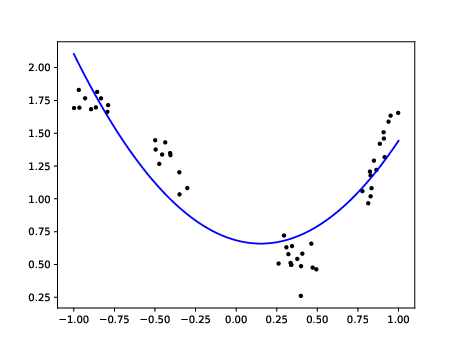
\includegraphics[width=0.32\textwidth]{images/Task1b_2_1.png}
                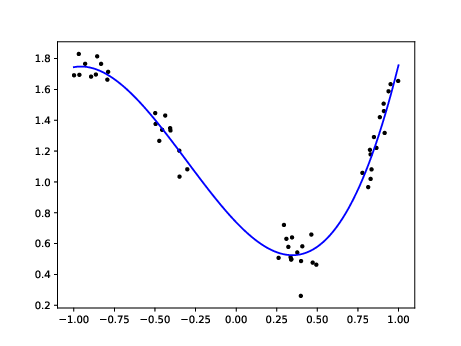
\includegraphics[width=0.32\textwidth]{images/Task1b_2_2.png}
                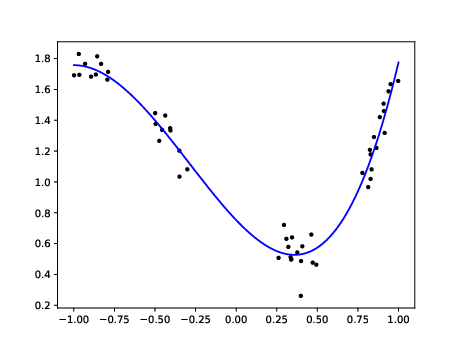
\includegraphics[width=0.32\textwidth]{images/Task1b_2_3.png}
                \caption{Polynomial ridge regression fits with degrees 2 (left), 3 (center), and 4 (right).}
            \end{figure}

            The degree 2 model captures the general U-shape trend but misses the fine details on the ends.
            The degree 3 model fits the data much more accurately.
            The degree 4 model performs similarly to degree 3, with no relevant visual differences.
            The improvement from degree 2 to 3 is significant, while the gain from degree 3 to 4 is minor.

            \vspace{2em}

            \textbf{3. Why do we call this method \textit{linear} regression despite using polynomials?}

            Even though we use polynomial functions of the input, the model is still linear in the parameters $w$.
            The prediction is a weighted sum of the features, and we do not multiply or compose the parameters.
            That’s why it's still called linear regression.

            \[
            f(x) = w^\top \phi(x) = w_0 + w_1 x + w_2 x^2 + \dots + w_d x^d
            \]
        \end{solution}
    \end{subtask}

    \begin{subtask}[points=10, title=Bayesian Linear Regression]
        Implement Bayesian linear ridge regression by filling in the ToDos of the corresponding task in the provided Colab Template. Assuming that $\mathbf{w}$ follows a multivariate Gaussian distribution, such that
        
        \begin{equation*}
            \mathbf{w} \sim \mathcal{N}(\bm{\mu}_0, \bm{\Lambda}_0^{-1}),
        \end{equation*}

        where ridge regression dictates $\bm{\mu}_0 = \mathbf{0}$ and $\bm{\Lambda}_0 = \lambda \mathbf{I}$.

        Here, $\bm{\mu}_0$ is the prior weight mean and $\bm{\Lambda}_0$ is the prior weight precision matrix, i.e.~the inverse of the covariance matrix.
        The corresponding posterior parameters can be denoted as $\bm{\mu}_n$ and $\bm{\Lambda}_n$.

        Assume $\sigma = 0.1$, use $\lambda = 0.01$, and
        include an additional input dimension to represent a bias term.
        Use all of the provided training data for a single Bayesian update.

        \begin{enumerate}
            \item State the posterior distribution of the model parameters $p(\mathbf{w} \mid \mathbf{X}, \mathbf{y})$ (no derivation required). 
            \item State the predictive distribution $p(\mathbf{y}_* \mid \mathbf{X}_*, \mathbf{X}, \mathbf{y})$ (no derivation required). 
            \item Report the RMSE of the train and test data under your Bayesian model (use the predictive mean). 
            \item Report the average log-likelihood of the train and test data under your Bayesian model.
            \item Include the resulting plot and a short description. 
            \item Explain the differences between linear regression and Bayesian linear regression.
        \end{enumerate}

        \begin{solution}
            \textbf{1. State the posterior distribution of the model parameters $\bm{p(w | X, y)}$ (no derivation required).}

            We place a Gaussian prior on the weight vector:

            \[
            w \sim \mathcal{N}(0, \lambda^{-1} I)
            \]

            Given the likelihood
            
            \[
            p(y \mid X, w) = \mathcal{N}(y \mid \Phi w, \sigma^2 I)
            \]
            
            and the prior, we compute the posterior using Bayes' rule:
            
            \[
            p(w \mid X, y) \propto p(y \mid X, w)\, p(w)
            \]

            Because both the likelihood and prior are Gaussian, the posterior is also Gaussian:
            
            \[
            p(w \mid X, y) = \mathcal{N}(w \mid \mu, \Lambda^{-1})
            \]

            where the parameters are:

            \[
            \Lambda = \lambda I + \frac{1}{\sigma^2} \Phi^\top \Phi,
            \qquad
            \mu = \frac{1}{\sigma^2} \Lambda^{-1} \Phi^\top \mathbf{y}
            \]

            \vspace{2em}

            \textbf{2. State the predictive distribution $\bm{p(y_* | X_*, X, y)}$ (no derivation required).}

            For a new input $x_*$, the output $y_*$ is also Gaussian-distributed, even after marginalizing over the uncertainty in $w$:
            
            \[
            p(y_* \mid x_*, X, y) = \int p(y_* \mid x_*, w)\, p(w \mid X, y)\, dw
            \]

            Both terms are Gaussian, so the result is Gaussian as well:
            
            \[
            p(y_* \mid x_*, X, y) = \mathcal{N}(y_* \mid \mu^\top \phi(x_*),\ \sigma^2 + \phi(x_*)^\top \Lambda^{-1} \phi(x_*))
            \]

            The mean and variance of the predictive distribution is:
            
            \[
            \mathbb{E}[y^*] = \mu^\top \phi(x^*)
            \qquad
            \text{Var}(y^*) = \sigma^2 + \phi(x^*)^\top \Lambda^{-1} \phi(x^*)
            \]

            \vspace{2em}

            \textbf{3. Report the RMSE of the train and test data under your Bayesian model (use the predictive mean).}

            The result of the RMSE of the train and test data for the Bayesian Linear Regression is:

            \vspace{1em}

            \textbf{\texttt{Bayesian Linear Regression}}
            \begin{itemize}
                \item \texttt{Train RMSE: 0.4122}
                \item \texttt{Test RMSE: 0.3843}
            \end{itemize}

            \vspace{1em}

            These RMSE values are the same as those obtained from the linear ridge regression model, since the predictive mean of the Bayesian model corresponds exactly to the ridge solution in this case.
            This confirms the theoretical equivalence between MAP estimation and Bayesian inference using Gaussian priors and likelihoods.

            \vspace{2em}

            \textbf{4. Report the average log-likelihood of the train and test data under your Bayesian model.}

            \begin{itemize}
                \item \texttt{Average Train Log-LLH: -27568.08}
                \item \texttt{Average Test Log-LLH: -25265.41}
            \end{itemize}

            \vspace{1em}

            These values indicate the model's overall likelihood fit.
            While the absolute values are negative due to the log of probabilities, closer values between train and test indicate reasonable generalization.

            \vspace{2em}

            \textbf{5. Include the resulting plot and a short description.}

            \begin{figure}[H]
                \centering
                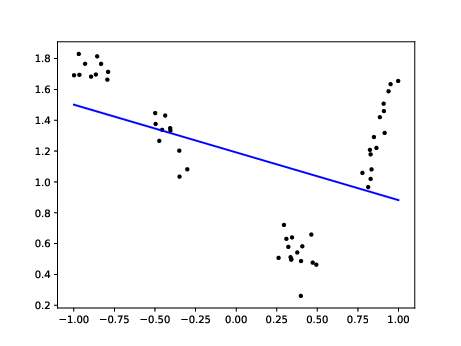
\includegraphics[width=0.5\textwidth]{images/Task1c_5.png}
                \caption{Bayesian linear regression fit with predictive mean and linear features.}
            \end{figure}

            The model fits a straight line with the predictive mean.
            Since the underlying function is nonlinear, the model underfits, but still captures a global trend.

            \vspace{2em}

            \textbf{6. Explain the differences between linear regression and Bayesian linear regression.}
        
            The key difference between these two regressions lies in how the model treats the weights:

            \begin{itemize}
                \item \textbf{Linear regression} finds a single point estimate for the weight vector $w$ by minimizing the squared loss (possibly with regularization).
                \item \textbf{Bayesian linear regression} treats $w$ as a random variable and infers a posterior distribution over it using Bayes' rule.
            \end{itemize}

            As a result:
            \begin{itemize}
                \item Linear regression produces a single prediction.
                \item Bayesian linear regression provides both a mean prediction and uncertainty (variance) around it.
            \end{itemize}

            Treating Bayesian as a probability allows models to quantify confidence in their predictions and to update beliefs as new data is observed.
        \end{solution}
    \end{subtask}

    \begin{subtask}[points=8, title=Squared Exponential Features]
        Implement Bayesian linear ridge regression using squared exponential (SE) features by filling in the ToDos of the corresponding task in the provided Colab Template.
        In other words, replace your observed data matrix $\mathbf{X} \in \mathbb{R}^{n \times 1}$ by a feature matrix $\bm{\Phi} \in \mathbb{R}^{n \times k}$, where

        \begin{equation*}
            \bm{\Phi}_{ij} = \exp \left( -\frac{1}{2} \beta (\mathbf{X}_i - \alpha_j)^2 \right).
        \end{equation*}

        Set $k = 20$, $\alpha_j = j * 0.1 - 1$ and $\beta = 10$. Use the ridge coefficient $\lambda = 0.01$ and assume known Gaussian noise with $\sigma = 0.1$.
        Include an additional input dimension to represent a bias term.

        \begin{enumerate}
            \item Report the RMSE of the train and test data under your Bayesian model with SE features. 
            \item Report the average log-likelihood of the train and test data under your Bayesian model with SE features. 
            \item Include the resulting plot and a short description. 
            \item How can SE features be interpreted from a statisticians point of view? What are $\alpha$ and $\beta$ in that context? 
        \end{enumerate}

        \begin{solution}

            \textbf{1. Report the RMSE of the train and test data under your Bayesian model with SE features.}

            \begin{itemize}
                \item \texttt{Train RMSE: 0.0816}
                \item \texttt{Test RMSE: 0.1434}
            \end{itemize}

            The RMSE values indicate a very accurate fit to the training data, and a adequate generalization performance on the test data.
            The improvement over the linear and polynomial features suggests that the SE features capture the local structure of the function well.

            \vspace{2em}

            \textbf{2. Report the average log-likelihood of the train and test data under your Bayesian model with SE features.}

            \begin{itemize}
                \item \texttt{Average Train Log-LLH: -244.12}
                \item \texttt{Average Test Log-LLH: -225.88}
            \end{itemize}

            These values indicate a high likelihood fit on both training and testing data, significantly better than the linear model.
            The SE features allow the model to express nonlinear patterns, leading to improved log-likelihood scores and better uncertainty estimates.

            \vspace{2em}

            \textbf{3. Include the resulting plot and a short description.}

            \begin{figure}[H]
                \centering
                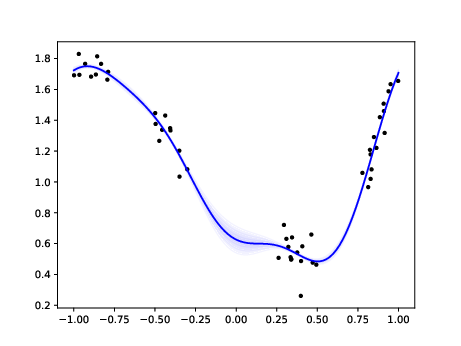
\includegraphics[width=0.5\textwidth]{images/Task1d_3.png}
                \caption{Bayesian regression with squared exponential features ($k=20$, $\beta=10$).}
            \end{figure}

            The blue curve represents the predictive mean, while the shaded area indicates the uncertainty.
            The fit is smooth and accurate across the entire input space, capturing both the global trend and local variations.

            \vspace{2em}

            \textbf{4. How can SE features be interpreted from a statisticians point of view? What are α and β in that context?}

            From a statistician’s perspective, they serve as a form of kernel feature transformation, mapping scalar inputs into a higher-dimensional feature space where each dimension captures similarity to a fixed center.

            Each feature is of the form:

            \[
            \phi_j(x) = \exp\left(-\frac{1}{2} \beta (x - \alpha_j)^2\right)
            \]

            Here:
            \begin{itemize}
                \item $\alpha_j$ defines the center of the $j$-th Gaussian basis function.
                \item $\beta$ controls the width of the basis function; it is the inverse of the variance and determines how local or global the feature response is.
            \end{itemize}

            By combining multiple SE features, the model can approximate complex nonlinear functions while maintaining interpretability and smoothness.

        \end{solution}
    \end{subtask}
\end{task}

% \newpage

% \begin{task}[points=12]{Gaussian Processes}
%     \begin{programmingtaskbox}
%         Google Collab:
%     \end{programmingtaskbox}

%     \begin{subtask}[title=GP Regression, points= 10]
%         Implement a Gaussian Process to fit the target function $y = \sin(x) + \cos^2(x)$ with $x \in [0, 0.005, 0.01, 0.015, \ldots, 2\pi]$. First, complete the function \texttt{rbf\_kernel()}.

%         Use the RBF/Gaussian kernel with a kernel bandwidth of 1, an initial mean of 0 and assume a noise variance of 0.005. Begin with no target data points and, at each iteration, sample a new point from the target function according to the uncertainty of your GP (that is, sample the point where the uncertainty is the highest) and update it. 

%         Plot your GP (mean and two times the standard deviation) after iterations 1, 2, 5, 10 and 15.
%         In each figure, plot also the true function as ground truth and add a new marker for each new sampled point. We have provided an example of the plot at iteration 4.

%         \textbf{Include the plots in your PDF submission.}

%         \begin{center}
%             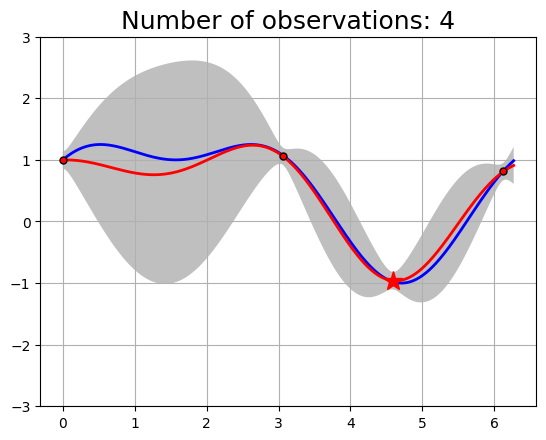
\includegraphics[scale=0.5]{gp_test_example.png}
%         \end{center}

%         Notes:
%         \begin{itemize}
%             \item The iteration number is equal to the number of sampled points, e.g. at iteration 5 there are 5 points sampled.
%             \item You do not need to strictly follow the given example plot, e.g., using different marker shapes or colors is okay.
%             \item The pyplot function \texttt{fill\_between()} might be useful to you.
%             \item For the RBF kernel, we use the definition on Slide 47, Lecture 6, where the vertical amplitude is set to 1.
%             \item If multiple points have the highest uncertainty, select the one with the lowest index in the dataset.
%         \end{itemize}

%         \begin{solution}

%         \end{solution}
%     \end{subtask}

%     \begin{subtask}[title=Kernel Parameters, points=2]
%         Explore various kernel hyperparameters, i.e., \texttt{rbf\_sigma} in the code, and explain how this parameter affects the prediction results.
        
%         \begin{solution}

%         \end{solution}
%     \end{subtask}
% \end{task}

% \newpage

% \begin{task}[points=28]{Principal Component Analysis}
% \begin{programmingtaskbox}
% Complete the corresponding section of the notebook as part of this task.
% \end{programmingtaskbox}
% In this exercise, you will use the dataset \texttt{iris.txt}. It contains data from three kind of Iris flowers (`Setosa', `Versicolour' and `Virginica') with 4 attributes: sepal length, sepal width, petal length, and petal width. Each row contains a sample while the last attribute is the label ($0$ means that the sample comes from a `Setosa' plant, $1$ from a `Versicolour' and $2$ from `Virginica').
% (You are allowed to use built-in functions for computing the mean, the covariance, eigenvalues and eigenvectors.)



% \begin{subtask}[points=3, title=Data Normalization]
% Normalizing the data is a common practice in machine learning. Normalize the provided dataset such that it has zero mean and unit variance per dimension. Why is normalizing important?
% Fill in the ToDos of the corresponding task in the provided Colab Template.

% \begin{solution}

% \end{solution}

% \end{subtask}



% \begin{subtask}[points=8, title=Principal Component Analysis]
% Apply PCA on your normalized dataset and generate a plot showing the proportion (percentage) of the cumulative variance explained (you can use the function \texttt{numpy.cumsum}). 
% How many components do you need in order to explain at least $95\%$ of the dataset variance? 
% Fill in the ToDos of the corresponding task in the provided Colab Template.
% \begin{solution}

% \end{solution}
% \end{subtask}



% \begin{subtask}[points=6, title=Low Dimensional Space]
% Using as many components as needed to explain $95\%$ of the dataset variance, generate a scatter plot of the lower-dimensional projection of the data. Use different colors or symbols for data points from different classes. Fill in the ToDos of the corresponding task in the provided Colab Template. What do you observe? 


% \begin{solution}

% \end{solution}

% \end{subtask}



% \begin{subtask}[points=6, title=Projection to the Original Space]
% Reconstruct the original dataset by using different number of principal components. Using the normalized root mean square error (NRMSE) as a metric, fill the table below (error per input versus the amount of principal components used). Fill in the ToDos of the corresponding task in the provided Colab Template.

% \begin{tabular}{c|r|r|r|r}
% N. of components & $x_1$ & $x_2$ & $x_3$ & $x_4$ \\
% \hline
% 1 & & & & \\
% 2 & & & & \\
% 3 & & & & \\
% 4 & & & &
% \end{tabular}

% Remember that in the first step you normalized the data.

% \begin{solution}

% \end{solution}
% \end{subtask}

% \newpage

% \begin{subtask}[points=5, title=Kernel PCA]
% Throughout this class we have seen that PCA is an easy and efficient way to reduce the dimensionality of some data. However, it is able to detect only linear dependences among data points. A more sophisticated extension to PCA, \emph{Kernel PCA}, is able to overcome this limitation. 
% This question asks you to deepen this topic by conducting some research by yourself: explain what Kernel PCA is, how it works and what are its main limitations. Be as concise (but clear) as possible.

% \begin{solution}

% \end{solution}
% \end{subtask}
% \end{task}

% \newpage

% \begin{task}[points=8]{Kernel Construction}
% Let \( X \) be a non-empty set. A \textbf{kernel} is a symmetric function \( k : X \times X \rightarrow \mathbb{R} \). The set \( X \) can have arbitrary structure (e.g., real vector space, graphs, images, strings, etc.). 

% A kernel \( k \) is called \textbf{positive definite} if for all finite subsets \( \{x_i\}_{i=1}^n \subseteq X \), the corresponding kernel matrix \( K \in \mathbb{R}^{n \times n} \) with entries \( K_{ij} = k(x_i, x_j) \) is positive semi-definite (check Lecture 6 slide 9), i.e.,

% \[
% \forall \alpha \in \mathbb{R}^n,\quad \alpha^\top K \alpha \geq 0.
% \]

% Let \( k_1, k_2 : X \times X \rightarrow \mathbb{R} \) be two positive definite kernels. We are to prove that the following operations yield valid positive definite kernels:

% \begin{enumerate}
%     \item \( k(x, x') = k_1(x, x') + k_2(x, x') \) 
%     \item \( k(x, x') = c \cdot k_1(x, x') \), for \( c \geq 0 \) 
%     \item \( k(x, x') = k_1(x, x') \cdot k_2(x, x') \) 
%     \item \( k(x, x') = k_1(f(x), f(x')) \) for some function \( f : X \rightarrow X \) 
% \end{enumerate}


% \begin{solution}

% \end{solution}


% \end{task}

\end{document}